\documentclass{beamer}
\usetheme{metropolis}
\usecolortheme{spruce}
\usepackage{amsmath}
\usepackage{tikz}
\usepackage{graphicx}
\usepackage{xcolor}
\usetikzlibrary{shapes,arrows,positioning,mindmap,trees,shadows,shapes.geometric}

% Custom colors
\definecolor{primary}{RGB}{41, 128, 185}
\definecolor{secondary}{RGB}{46, 204, 113}
\definecolor{accent}{RGB}{230, 126, 34}
\definecolor{neutral}{RGB}{52, 73, 94}
\definecolor{light}{RGB}{236, 240, 241}
\definecolor{nodeblue}{RGB}{41,128,185}
\definecolor{nodegray}{RGB}{149,165,166}

% Custom styles for diagrams
\tikzstyle{process} = [
    rectangle, 
    rounded corners=3mm, 
    minimum width=2.5cm, 
    minimum height=1cm, 
    text centered, 
    draw=primary,
    fill=light,
    drop shadow,
    font=\small
]

\tikzstyle{arrow} = [
    thick,
    -stealth,
    draw=neutral
]

\tikzstyle{tree} = [
    rectangle,
    rounded corners=3mm,
    minimum width=2cm,
    minimum height=0.8cm,
    text centered,
    draw=primary,
    fill=light,
    font=\small
]

% Presentation settings
\setbeamertemplate{navigation symbols}{}
\setbeamertemplate{footline}[frame number]
\setbeamerfont{title}{size=\Large,series=\bfseries}
\setbeamerfont{subtitle}{size=\large}

\title{Internal Analysis \& Target-Based Planning}
\subtitle{A Framework for Platform Development}
\date{\today}

\begin{document}

\begin{frame}
    \titlepage
\end{frame}

\begin{frame}{Overview}
    \begin{columns}[T,onlytextwidth]
        \column{0.48\textwidth}
        \begin{block}{Part I: Internal Analysis}
            \begin{itemize}
                \item Team Dependencies
                \item Flow Efficiency
                \item Distribution Models
                \item Cost Analysis
            \end{itemize}
        \end{block}
        
        \column{0.48\textwidth}
        \begin{block}{Part II: Target-Based Planning}
            \begin{itemize}
                \item Platform Solutions
                \item Investment Analysis
                \item Scenario Planning
                \item Optimization Strategy
            \end{itemize}
        \end{block}
    \end{columns}
\end{frame}

\section{Part I: Internal Analysis}

\begin{frame}{Dependency Analysis Framework}
    \begin{center}
    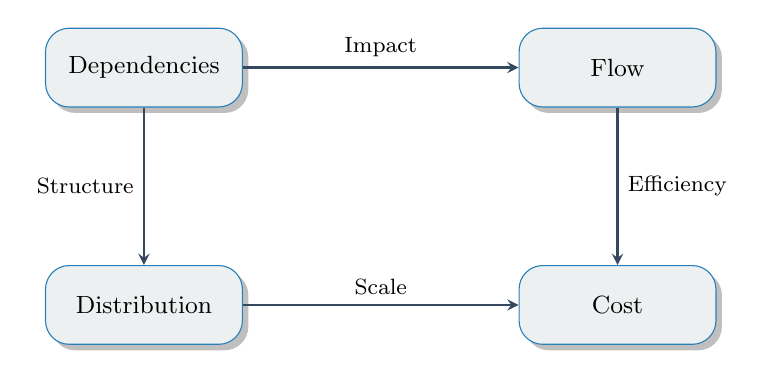
\begin{tikzpicture}[node distance=3.5cm]
        \node[process] (dep) {Dependencies};
        \node[process, right=of dep] (flow) {Flow};
        \node[process, below=2cm of dep] (dist) {Distribution};
        \node[process, below=2cm of flow] (cost) {Cost};
        
        \draw[arrow] (dep) -- (flow) 
            node[midway, above, font=\footnotesize] {Impact};
        \draw[arrow] (dep) -- (dist)
            node[midway, left, font=\footnotesize] {Structure};
        \draw[arrow] (flow) -- (cost)
            node[midway, right, font=\footnotesize] {Efficiency};
        \draw[arrow] (dist) -- (cost)
            node[midway, above, font=\footnotesize] {Scale};
    \end{tikzpicture}
    \end{center}
\end{frame}

\begin{frame}{Dependency Impact Score}
    \begin{columns}[T,onlytextwidth]
        \column{0.5\textwidth}
        \begin{equation*}
            DIS = \sum(W_i \times D_i \times C_i)
        \end{equation*}
        \begin{itemize}
            \item $W_i$: Volume weight
            \item $D_i$: Strength (1-5)
            \item $C_i$: Cost factor
        \end{itemize}
        
        \column{0.5\textwidth}
        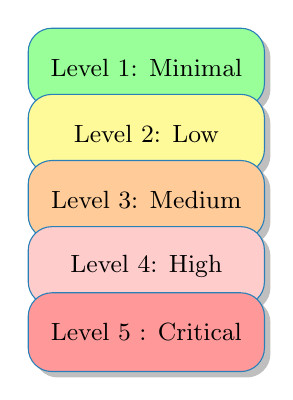
\begin{tikzpicture}[scale=0.7]
            \foreach \y/\c/\t/\l [count=\i] in {
                0/green!40/Minimal/1,
                1/yellow!40/Low/2,
                2/orange!40/Medium/3,
                3/red!20/High/4,
                4/red!40/Critical/5
            } {
                \node[process, fill=\c, minimum width=3cm] 
                    at (0,-\y*1.2) {Level \l: \t};
            }
        \end{tikzpicture}
    \end{columns}
\end{frame}

\begin{frame}{Flow Efficiency Model}
    \begin{center}
    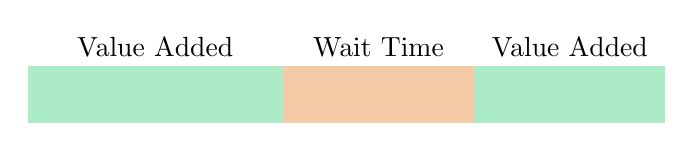
\begin{tikzpicture}[scale=0.9]
        % Timeline bar
        \fill[light] (0,0) rectangle (9,0.8);
        \fill[secondary!40] (0,0) rectangle (3.6,0.8);
        \fill[accent!40] (3.6,0) rectangle (6.3,0.8);
        \fill[secondary!40] (6.3,0) rectangle (9,0.8);
        
        % Labels
        \node[above] at (1.8,0.8) {Value Added};
        \node[above] at (4.95,0.8) {Wait Time};
        \node[above] at (7.65,0.8) {Value Added};
    \end{tikzpicture}
    \end{center}
    
    \vspace{0.3cm}
    \begin{equation*}
        FE = \frac{\sum \text{Value Added Time}}{\sum \text{Total Lead Time}} \times 100\%
    \end{equation*}
    
    \begin{itemize}
        \item Target: $\text{FE} \geq 40\%$
        \item Identifies process waste
        \item Guides optimization efforts
    \end{itemize}
\end{frame}

\begin{frame}{Distribution Models}
    \begin{columns}[T,totalwidth=\textwidth]
        \begin{column}{0.48\textwidth}
            \centering
            \textbf{\large Even Distribution}
            \vspace{0.3cm}
            
            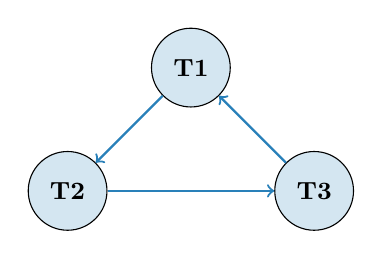
\begin{tikzpicture}[
                node distance=1.8cm,
                every node/.style={
                    draw,
                    circle,
                    fill=nodeblue!20,
                    minimum size=1cm,
                    font=\small\bfseries
                }
            ]
                \node (A) {T1};
                \node (B) [below left=1.2cm of A] {T2};
                \node (C) [below right=1.2cm of A] {T3};
                \draw[->, thick, nodeblue] (A) -- (B);
                \draw[->, thick, nodeblue] (B) -- (C);
                \draw[->, thick, nodeblue] (C) -- (A);
            \end{tikzpicture}
            
            \vspace{0.3cm}
            \begin{itemize}
                \item[\textcolor{nodeblue}{$\bullet$}] Equal responsibilities
                \item[\textcolor{nodeblue}{$\bullet$}] Direct communication
                \item[\textcolor{nodeblue}{$\bullet$}] Balanced load
            \end{itemize}
        \end{column}
        
        \begin{column}{0.48\textwidth}
            \centering
            \textbf{\large Hub and Spoke}
            \vspace{0.3cm}
            
            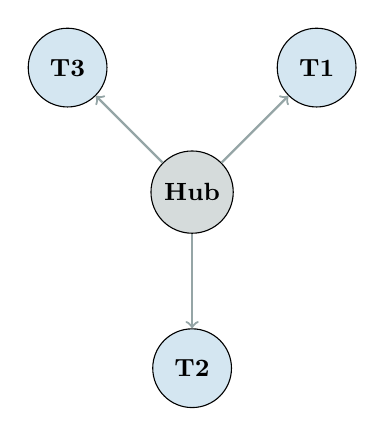
\begin{tikzpicture}[
                node distance=1.8cm,
                every node/.style={
                    draw,
                    circle,
                    minimum size=1cm,
                    font=\small\bfseries
                },
                spoke/.style={
                    fill=nodeblue!20
                },
                hub/.style={
                    fill=nodegray!40
                }
            ]
                \node[hub] (H) {Hub};
                \node[spoke] (A) [above right=1.2cm of H] {T1};
                \node[spoke] (B) [below=1.2cm of H] {T2};
                \node[spoke] (C) [above left=1.2cm of H] {T3};
                \draw[->, thick, nodegray] (H) -- (A);
                \draw[->, thick, nodegray] (H) -- (B);
                \draw[->, thick, nodegray] (H) -- (C);
            \end{tikzpicture}
            
            \vspace{0.3cm}
            \begin{itemize}
                \item[\textcolor{nodegray}{$\bullet$}] Centralized control
                \item[\textcolor{nodegray}{$\bullet$}] Streamlined flow
                \item[\textcolor{nodegray}{$\bullet$}] Clear hierarchy
            \end{itemize}
        \end{column}
    \end{columns}
\end{frame}

\begin{frame}{Cost Structure}
    \begin{center}
    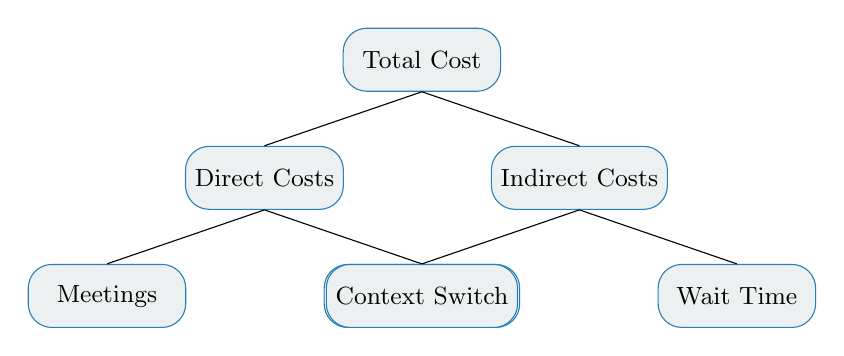
\begin{tikzpicture}[
        grow=down,
        sibling distance=4cm,
        level distance=1.5cm,
        edge from parent path={(\tikzparentnode.south) -- (\tikzchildnode.north)}
    ]
        \node[tree] {Total Cost}
            child {
                node[tree] {Direct Costs}
                child {node[tree] {Meetings}}
                child {node[tree] {Communication}}
            }
            child {
                node[tree] {Indirect Costs}
                child {node[tree] {Context Switch}}
                child {node[tree] {Wait Time}}
            };
    \end{tikzpicture}
    \end{center}
    
    \vspace{0.3cm}
    \begin{equation*}
        AC = BC \times (1 + DF)
    \end{equation*}
    where $DF = \text{deps} \times 0.15$
\end{frame}

\section{Part II: Target-Based Planning}

\begin{frame}{Target-Based Approach}
    \begin{center}
    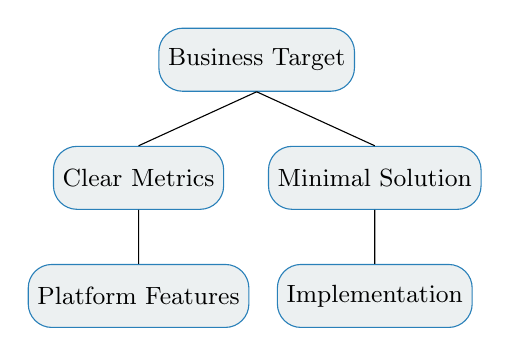
\begin{tikzpicture}[
        grow=down,
        level distance=1.5cm,
        sibling distance=3cm,
        edge from parent path={(\tikzparentnode.south) -- (\tikzchildnode.north)}
    ]
        \node[tree] {Business Target}
            child {
                node[tree] {Clear Metrics}
                child {node[tree] {Platform Features}}
            }
            child {
                node[tree] {Minimal Solution}
                child {node[tree] {Implementation}}
            };
    \end{tikzpicture}
    \end{center}
    
    \vspace{0.5cm}
    \begin{itemize}
        \item Start with business outcomes
        \item Define clear metrics
        \item Design minimal features
        \item Implement iteratively
    \end{itemize}
\end{frame}

\begin{frame}{Platform Solutions}
    \begin{columns}[T,onlytextwidth]
        \column{0.48\textwidth}
        \begin{block}{Team-Based Platform}
            \begin{center}
            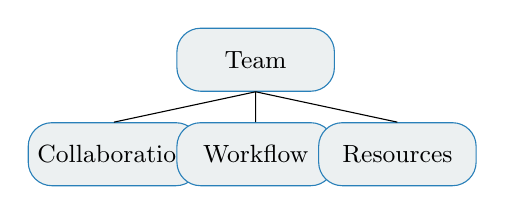
\begin{tikzpicture}[
                grow=down,
                sibling distance=1.8cm,
                level distance=1.2cm,
                edge from parent path={(\tikzparentnode.south) -- (\tikzchildnode.north)}
            ]
                \node[tree] {Team}
                    child {node[tree] {Collaboration}}
                    child {node[tree] {Workflow}}
                    child {node[tree] {Resources}};
            \end{tikzpicture}
            \end{center}
        \end{block}
        
        \column{0.48\textwidth}
        \begin{block}{Ticket-Based Platform}
            \begin{center}
            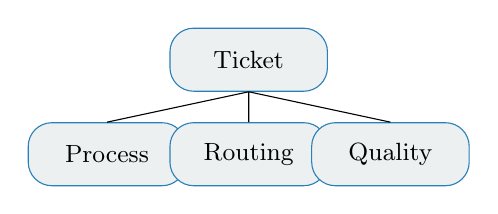
\begin{tikzpicture}[
                grow=down,
                sibling distance=1.8cm,
                level distance=1.2cm,
                edge from parent path={(\tikzparentnode.south) -- (\tikzchildnode.north)}
            ]
                \node[tree] {Ticket}
                    child {node[tree] {Process}}
                    child {node[tree] {Routing}}
                    child {node[tree] {Quality}};
            \end{tikzpicture}
            \end{center}
        \end{block}
    \end{columns}
\end{frame}

\begin{frame}{Investment Analysis}
    \begin{center}
    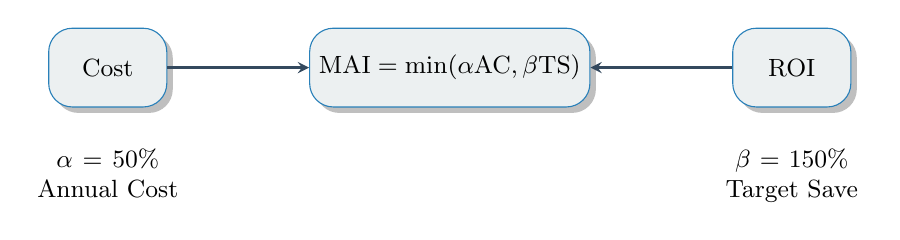
\begin{tikzpicture}[
        node distance=1.8cm,
        every node/.style={
            font=\small
        }
    ]
        \node[process, minimum width=2.8cm] (mai) {$\text{MAI} = \min(\alpha\text{AC}, \beta\text{TS})$};
        \node[process, minimum width=1.5cm, left=of mai] (cost) {Cost};
        \node[process, minimum width=1.5cm, right=of mai] (roi) {ROI};
        
        \draw[arrow] (cost) -- (mai);
        \draw[arrow] (roi) -- (mai);
        
        \node[below=0.4cm of cost, text width=1.8cm, align=center] {
            $\alpha = 50\%$\\Annual Cost
        };
        \node[below=0.4cm of roi, text width=1.8cm, align=center] {
            $\beta = 150\%$\\Target Save
        };
    \end{tikzpicture}
    \end{center}
    
    \vspace{0.2cm}
    \begin{itemize}
        \item MAI: Maximum Allowable Investment
        \item AC: Annual Cost
        \item TS: Target Savings
    \end{itemize}
\end{frame}

\begin{frame}{Scenario Analysis}
    \begin{center}
    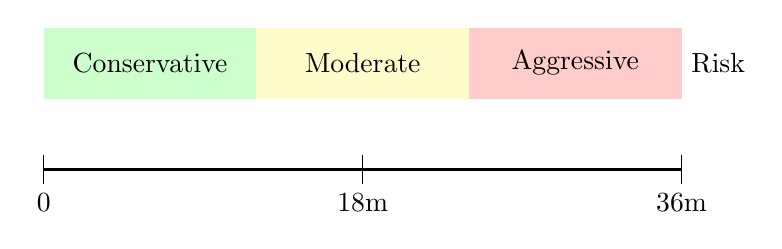
\begin{tikzpicture}[scale=0.9]
        % Timeline axis
        \draw[thick] (0,0) -- (9,0);
        \foreach \x/\t in {0/0, 4.5/18m, 9/36m} {
            \draw (\x,-0.2) -- (\x,0.2);
            \node[below] at (\x,-0.2) {\t};
        }
        
        % Scenarios
        \fill[green!20] (0,1) rectangle (3,2);
        \fill[yellow!20] (3,1) rectangle (6,2);
        \fill[red!20] (6,1) rectangle (9,2);
        
        \node at (1.5,1.5) {Conservative};
        \node at (4.5,1.5) {Moderate};
        \node at (7.5,1.5) {Aggressive};
        
        % Risk levels
        \node[right] at (9,1.5) {Risk};
    \end{tikzpicture}
    \end{center}
    
    \vspace{0.3cm}
    \begin{columns}[T,onlytextwidth]
        \column{0.32\textwidth}
        \begin{itemize}
            \item Time: $-10\%$
            \item Quality: $+15\%$
            \item ROI: 24m
        \end{itemize}
        
        \column{0.32\textwidth}
        \begin{itemize}
            \item Time: $-20\%$
            \item Quality: $+25\%$
            \item ROI: 18m
        \end{itemize}
        
        \column{0.32\textwidth}
        \begin{itemize}
            \item Time: $-30\%$
            \item Quality: $+35\%$
            \item ROI: 12m
        \end{itemize}
    \end{columns}
\end{frame}

\section{Conclusion}

\begin{frame}{Key Takeaways}
    \begin{columns}[T,onlytextwidth]
        \column{0.48\textwidth}
        \begin{block}{Benefits}
            \begin{itemize}
                \item Data-driven decisions
                \item Clear metrics
                \item Risk management
                \item Adaptable approach
            \end{itemize}
        \end{block}
        
        \column{0.48\textwidth}
        \begin{block}{Next Steps}
            \begin{itemize}
                \item Choose platform type
                \item Set specific targets
                \item Design minimal solution
                \item Measure outcomes
            \end{itemize}
        \end{block}
    \end{columns}
\end{frame}

\end{document} 